\chapter{Referencial Teórico}
Nesta seção, serão apresentados os fundamentos teóricos que servirão de base para sustentar o estudo sobre a inteligência
artificial dentro da área de algoritmos e motores do jogo de xadrez para computador. Primeiramente, iremos compreender as
teorias e conceitos de base para esta pesquisa, que proveram as informações necessárias para a análise e comparação em questão.
Depois, falaremos sobre o estado da arte deste tema.

\section{Teoria e Conceitos de Base}
Esta parte do projeto conterá as informações teóricas necessárias para compreensão do tema e sua problematização,
assim veremos os conceitos de inteligência artificial, motor de xadrez, algoritmo de busca \textit{min-max},
algoritmo \textit{alpha-beta pruning} e suas funções com uso de redes neurais.

\subsection{Conceito de Inteligencia Artificial}
O conceito de inteligência artificial surgiu da ideia de reproduzir nas máquinas a capacidade humana de usar das informações
disponíveis para resolver problemas e tomar decisões com base na razão e lógica, o que resultou em dar aos computadores a
capacidade de automatizar processos ou pelo menos minimizar consideravelmente o envolvimento humano nós mesmos,
e com o avanço cada vez maior da velocidade de processamento das máquinas, elas alcançaram a capacidade de analisar dados
em taxas extremamente mais rápidas do que a humana.

Hintze (2016) nos explica sobre os tipos mais básicos da inteligência artificial,
\begin{citacao}
    Os tipos mais básicos de sistemas de IA são puramente reativos e não têm a capacidade de formar memórias nem de usar
    experiências passadas para informar as decisões atuais. Deep Blue, o supercomputador de xadrez da IBM, que derrotou o
    grande mestre internacional Garry Kasparov no final dos anos 1990, é o exemplo perfeito desse tipo de máquina.
    \cite[tradução nossa.]{HINTZE}
\end{citacao}

Também é dito por Jajal (2018) que:
\begin{citacao}
    A Inteligência Artificial Estreita (AIE) também conhecida como IA “fraca” é a IA que existe em nosso mundo hoje.
    AIE é a IA programada para realizar uma única tarefa – seja verificar o clima, jogar xadrez ou analisar dados brutos
    para escrever relatórios jornalísticos.\cite[tradução nossa.]{JAJAL}
\end{citacao}

É importante diferenciar o tipo mais básico de inteligência artificial dos mais complexos, pois o pensamento mais comum
quando falamos neste tema é a criação de máquinas semelhantes aos humanos que assim como nós possam pensar e agir por conta
própria, possuindo a capacidade de aprender e até mesmo possuir sentimentos e consciência, mas tais feitos só podem ser
alcançados utilizando-se de tecnologias de áreas como machine learning e redes neurais, que são ramos da inteligência
artificial.

De acordo com Allende-Cid(2019),
\begin{citacao}
    Machine Learning é a área ideal para a automatização de processos, os quais podem ser "simples", como reconhecer padrões visuais, ou complexos,
    tais quais decisões de especialistas da área da saúde. Quando seres humanos lidam com problemas complexos, muitas vezes é impossível explicar o raciocínio
    que levou a tomar determinadas decisões. Por outro lado, é menos complexo realizarmos a coleta dos exemplos de decisões tomadas por seres humanos e usá-los
    como fonte para que o sistema aprenda a resolver o mesmo problema.\cite[tradução dos editores, p.16.]{ALLEND-CID}
\end{citacao}

\subsection{Conceito do motor de xadrez}
A primeira aplicação de um motor de xadrez foi criada entre os anos de 1950 a 1953 por Alan Turing juntamente com a ideia base
de Claude Shannon, criando assim o primeiro algoritmo para o jogo de xadrez de computador, que pela falta de uma máquina
adequada teve que ter cada movimento calculado manualmente por Turing via o algoritmo.

Santana (2014) define um motor de xadrez como:
\begin{citacao}
    (...) um programa de computador capaz de decidir um movimento em uma partida de xadrez. Tal programa recebe uma
    configuração de um tabuleiro, isto é, o conjunto de casas contendo a informação de qual peça está ocupando cada casa,
    analisa esta informação considerando somente os movimentos válidos e retorna um movimento que é o melhor possível de
    acordo com algum critério.\cite[p.4.]{SANTANA2014}
\end{citacao}

Os motores de xadrez em geral não possuem interface gráfica própria, eles apenas recebem comandos e devolvem o próximo
movimento, assim para que haja interação com outros programas se faz necessário um protocolo de comunicação, a partir
da padronização de comandos utilizados no protocolo, dois motores diferentes podem interagir com uma mesma interface
sem conflitos.

É necessário que o motor faça a representação do tabuleiro do jogo, mantendo dados como a posição de todas as peças no tabuleiro,
a regra de 50 movimentos, entre outros. Uma boa representação do tabuleiro torna o cálculo de movimentos e a avaliação do tabuleiro
muito rápidas, de forma geral, existem três métodos diferentes para representar um tabuleiro: centrado nas casas, centrado nas peças
e soluções híbridas.

Bijl e Tiet (2021) ressaltam a importância desta fase, pois qualquer algoritmo, esteja relacionado a pesquisa
ou avaliação, tem como base a implementação da representação do tabuleiro.

\subsection{Algoritmo de busca min-max}

O minimax é um algoritmo de força bruta, isso significa que seu objetivo é enumerar todos os possíveis candidatos de uma solução e verificar
se cada um satisfaz o problema, no caso do minimax ele divide as possibilidades de ações de cada um dos jogadores em uma árvore de jogadas para
conseguir a melhor jogada possível.

Essa árvore vai ser definida em etapas de minimização(min) e maximização(max), sendo cada uma destas etapas representadas por uma jogada do
adversário ou da máquina respectivamente,o objetivo das jogadas de minimização é minimizar as chances de uma boa jogada da máquina e as de
maximização é maximizar as chances de uma boa jogada da máquina ocorrer,cada nó representa uma configuração do jogo, e cada aresta de um nó representa
uma jogada que leva a uma determinada configuração.

De acordo com Eric Thé(1992):
\begin{citacao}
    Jogos de soma-zero com dois jogadores que exigem inteligência humana como Xadrez, damas, go e othello
    podem ser todos resolvidos computacionalmente programando uma procurando uma busca computacional de
    arvore de estado-espaço onde os nós representam o as posições do problema ou os estados (o tabuleiro do jogo)
    e os ramos representam as operações que transformam um estado em outro.\cite[tradução nossa.]{ERICTHE}
\end{citacao}

Nós que não possuem arestas são denominados de nó folha, esses nós são configurações de fim de jogo, são aplicados nesses nós um fator avaliativo
para validar se aquele nó possui um resultado positivo ou negativo para a máquina, o nó em questão recebe um valor com base no seu resultado.


No caso do xadrez o valor avaliativo é dado com base em um valor específico para cada peça, caso haja mais peças da máquina com um valor
significativo aquele  possui um valor positivo, caso contrário possui um valor negativo.

Após a avaliação todos as arestas de um nó atribuirmos um valor ao mesmo, se o nó em questão for um nó de min, ou seja, uma jogada
do adversário, atribuímos ao nó o valor mínimo entre os valores de suas arestas, caso seja o max, uma jogada da máquina, atribuímos
o valor máximo entre suas arestas.

No fim de todas as arestas o algoritmo escolhe a aresta com o maior valor pois esta é a melhor alternativa para se seguir.

\begin{figure}[!ht]
    \Caption{Representação do algoritmo minimax}
    \centering
    \label{minimax}
    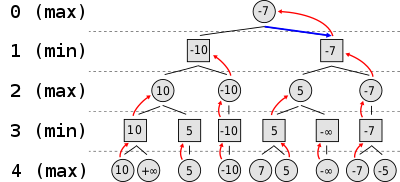
\includegraphics[scale=0.8]{figuras/minimax2.png}
    \Fonte{\url{https://wblog.wiki/pt/Minimax}. Acessado em: 24 de jun. 2022}
\end{figure}

\begin{figure}[!ht]
    \Caption{Representação do algoritmo minimax no xadrez}
    \centering
    \label{minimax-chess}
    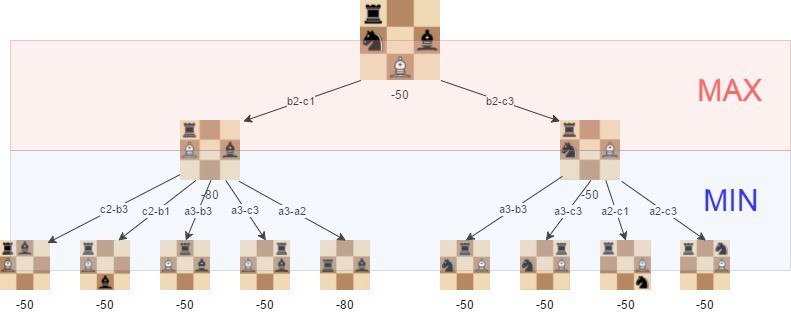
\includegraphics[scale=0.5]{figuras/Minimax Chess.jpeg}
    \Fonte{\url{https://www.freecodecamp.org/news/simple-chess-ai-step-by-step-1d55a9266977/}.\\ Acessado em: 24 de jun. 2022}
\end{figure}


\subsection{Algoritmo alpha-beta pruning}

O alpha-beta prunning é um algoritmo de otimização do minimax onde excluímos as arestas que possuem um valor
pior do que um valor encontrado anteriormente, isso é feito para economizar tempo de processamento da máquina
já que o algoritmo minimax por si só é muito custoso


O algoritmo funciona da seguinte forma,existem duas variáveis chamadas alpha e beta respectivamente,
alpha é o maior valor que o maximizador pode garantir naquele nível da árvore ou abaixo e beta é o menor
valor que o minimizador possui naquele nível da árvore ou abaixo, a cada subida na árvore esses valores são
atualizados com base nos maiores valores encontrados,logo,quando o algoritmo está decidindo o valor que irá
atribuir ao nó em questão ele verifica as variáveis para verificar se uma das arestas tem chances de possuir
um valor maior ou menor do que ele já possui nas variáveis alpha e beta.


Pegando por exemplo um nó maximizador A com dois nós filhos minimizadores,B e C,
caso o valor de B seja 6 saberemos que o nó A maximizador escolherá um valor maior ou igual a 6,
se avaliarmos o nó C e ele possuir um nó filho com valor 4, saberemos que aquele nó só escolherá um valor 4
ou menor, logo não há necessidade de fazer mais nenhuma avaliação de seus filhos pois o maior valor para o nó
A já foi escolhido.

\subsection{Funções com uso de redes neurais}

Redes neurais ou redes neurais artificiais é um dos tipos de machine learning que se inspira no cérebro
humano imitando a forma como os nossos neurônios conversam entre si usando um algoritmo de aprendizagem
que tem como objetivo modificar pesos sinápticos da rede de uma forma ordenada para alcançar uma solução esperada.

Haykin define redes neurais e suas semelhanças com o cérebro humano da seguinte forma:

\begin{citacao}
    Uma rede neural é um processador maciçamente paralelamente distribuído constituído de unidade de processamento simples,
    que têm a propensão natural para armazenar conhecimento experimental e torna-lo disponível para uso. Ela se assemelha ao cérebro humano
    em dois aspectos:

    1. O conhecimento é adquirido pela rede a partir de seu ambiente através de um processo de aprendizagem.

    2. Forças de conexão de neurônios, conhecidas como pesos sinápticos, são utilizados para armazenar o conhecimento adquirido.
    \cite{HAYKIN}
\end{citacao}

Fausett(1993) complementa dizendo que:
\begin{citacao}
    (...) um sistema de processamento de informações que possui certas características de desempenho em comum com as redes
    neurais biológicas. Redes neurais artificiais foram desenvolvidas como generalização de modelos matemáticos da cognição
    humana ou biologia neural (...) \cite[tradução nossa, p.3]{FAUSETT}
\end{citacao}

\subsection{Estado da Arte}

Existem vários trabalhos envolvendo a criação de motores de xadrez e descrição de seus algoritmos, iremos aqui citar
alguns dos quais tomamos como base para este projeto.

Santana (2014) apresenta teorias e algoritmos relacionados ao xadrez para computador e mostra possíveis implementações
para um motor de xadrez, no final ele analisa a implementação dentro do motor de xadrez de código aberto Pulse.

Abreu et al. (2006) também apresenta teorias e implementações de algoritmos, mas este descreve técnicas mais avançadas,
como: Tabelas de transposição, extensões e reduções de busca, livro de aberturas e banco de dados finais. Além disso,
este trabalho faz a análise resumida de um motor de xadrez de propriedade dos autores chamado ICE.

Block et al. (2008) apresenta a teoria matemática e lógica para implementar aprendizado por reforço por meio de um
método chamado Diferença Temporal (DT), o qual otimiza as funções de avaliação e seus coeficientes, e tem a capacidade
de aumentar sua própria compreensão do xadrez após cada partida.

Bijl e Tiet (2021) nos expõem uma visão mais atual quanto ao uso de alguns algoritmos em motores de xadrez. Eles fazem
a comparação de diferentes técnicas tanto no fator de velocidade quanto no de qualidade de movimentos.

Como pode ser visto, existem vários trabalhos explicando diferentes tipos de implementação dos algoritmos para motores de xadrez,
mas não muitos fazem a comparação entre eles e suas implementações nestes, assim buscamos ampliar a visão neste tema, mostrando
caminhos no qual os algoritmos podem ser melhorados.
